As we described above, our users need the UI of the project to be as easy and familiar to them as possible, because they will use it in critical situations, such as a parent describes the criminal who kidnapped his/her child. So, we tried to make the both Frontend Design and Backend Endpoints to be very simple and isolated from the complex techniques used in the background.

\subsubsection{Functional Description}
Our Application allows the user to get his/her intended face based on different generation modes that he/she can navigate through in the main page. Our generation modes are
\begin{itemize}
    \item Generation from Voice Description.
    \item Generation from Textual Description.
    \item Generation using Manual Manipulators.
\end{itemize}
After each mode, the user is allowed to do extra sequential refinements using manual manipulators and to generate 8 different head poses of the final refined face.

\subsubsection{Modular Decomposition}
As shown in figure \ref{fig:app}, we can decompose this module into two sub-modules, frontend design (\emph{user interface}) and backend API (\emph{server}).

\paragraph{Frontend Design}
We used VueJS as our frontend framework with Axios as a request handler. Our frontend design consists of 6 pages

\begin{itemize}
    \item Main Page
    
    This Page is just a page with single list of generation modes as shown in figure \ref{fig:main}
    
    \begin{figure}[H]
        \centering
        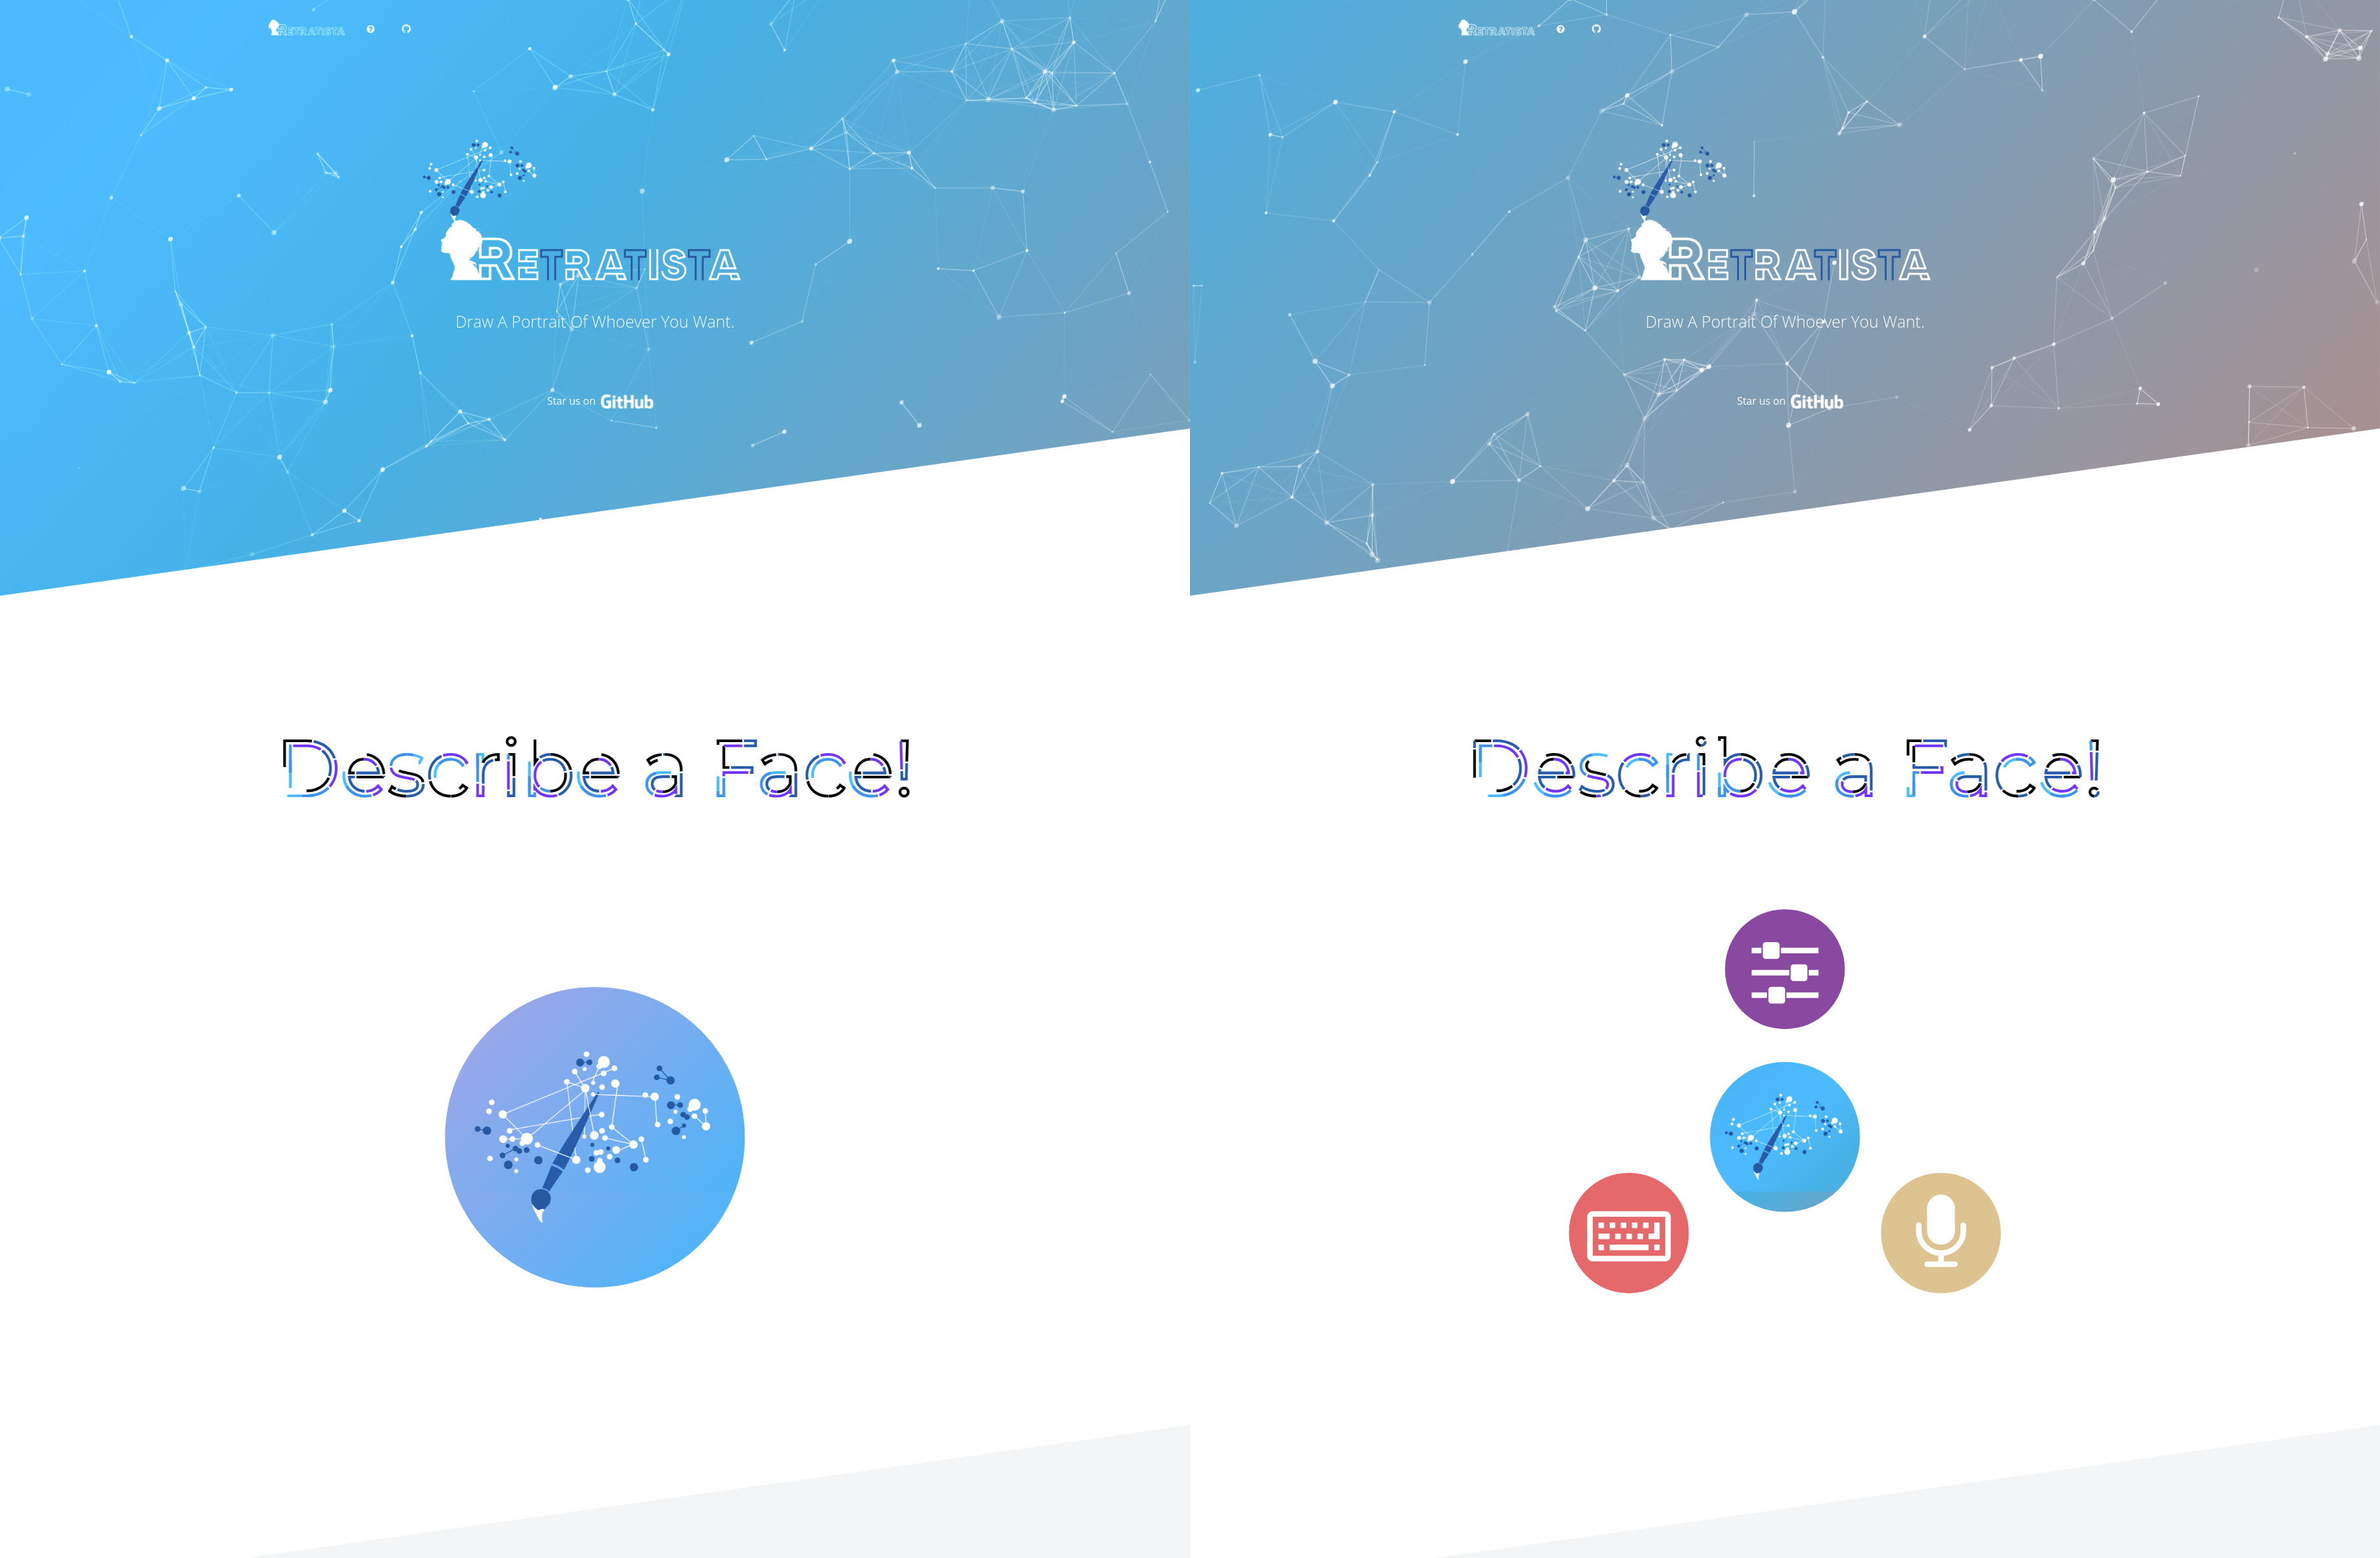
\includegraphics[width=0.6\textwidth]{images/website/mainpage.jpg}
        \caption{Main Page}
        \label{fig:main}
    \end{figure}
    
    \item Generation From Voice Description Page
    
    This Page is a page with two different assets (voice and textual input) for the user to describe a face. After generation, it allows the user to refine the generated face or generate head poses, as shown in figure \ref{fig:voice}
    
    \begin{figure}[H]
        \centering
        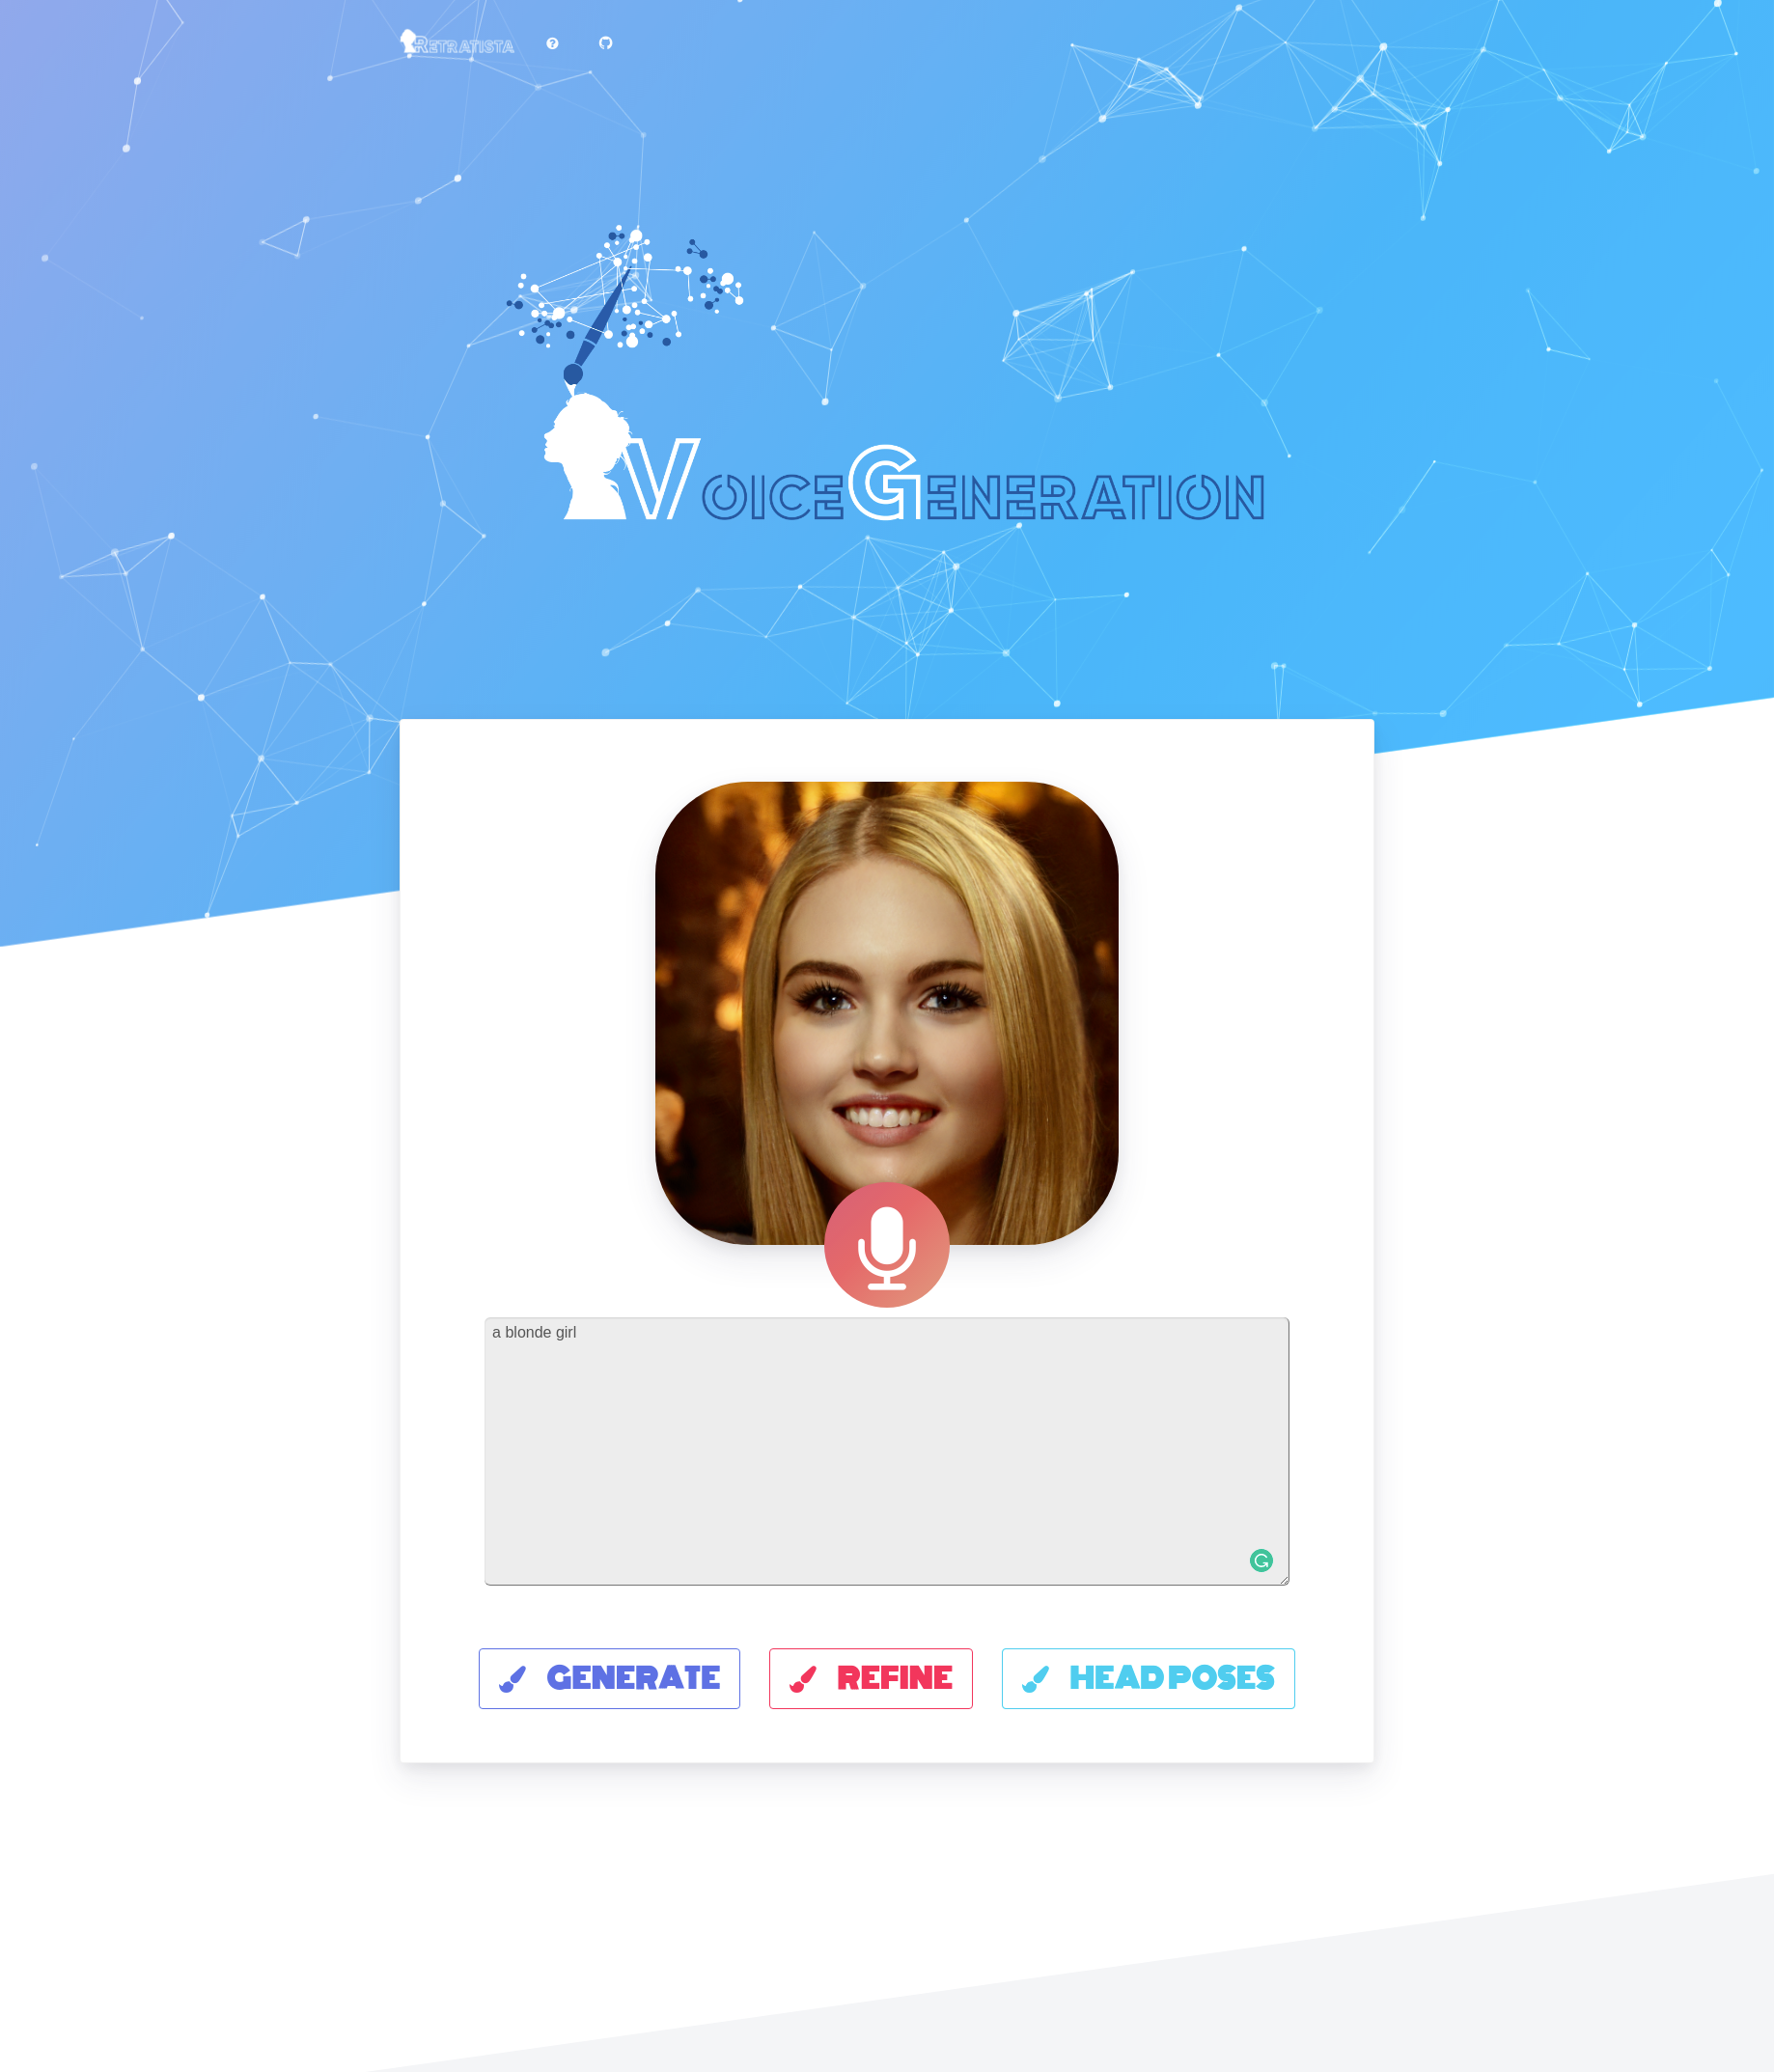
\includegraphics[width=0.7\textwidth]{images/website/voice.png}
        \caption{Generation From Voice Description Page}
        \label{fig:voice}
    \end{figure}
    
    
    \item Generation From Textual Description Page
    
    This Page is a page with one asset (textual input) for the user to describe a face. After generation, it allows the user to refine the generated face or generate head poses, as shown in figure \ref{fig:text}
    
    \begin{figure}[H]
        \centering
        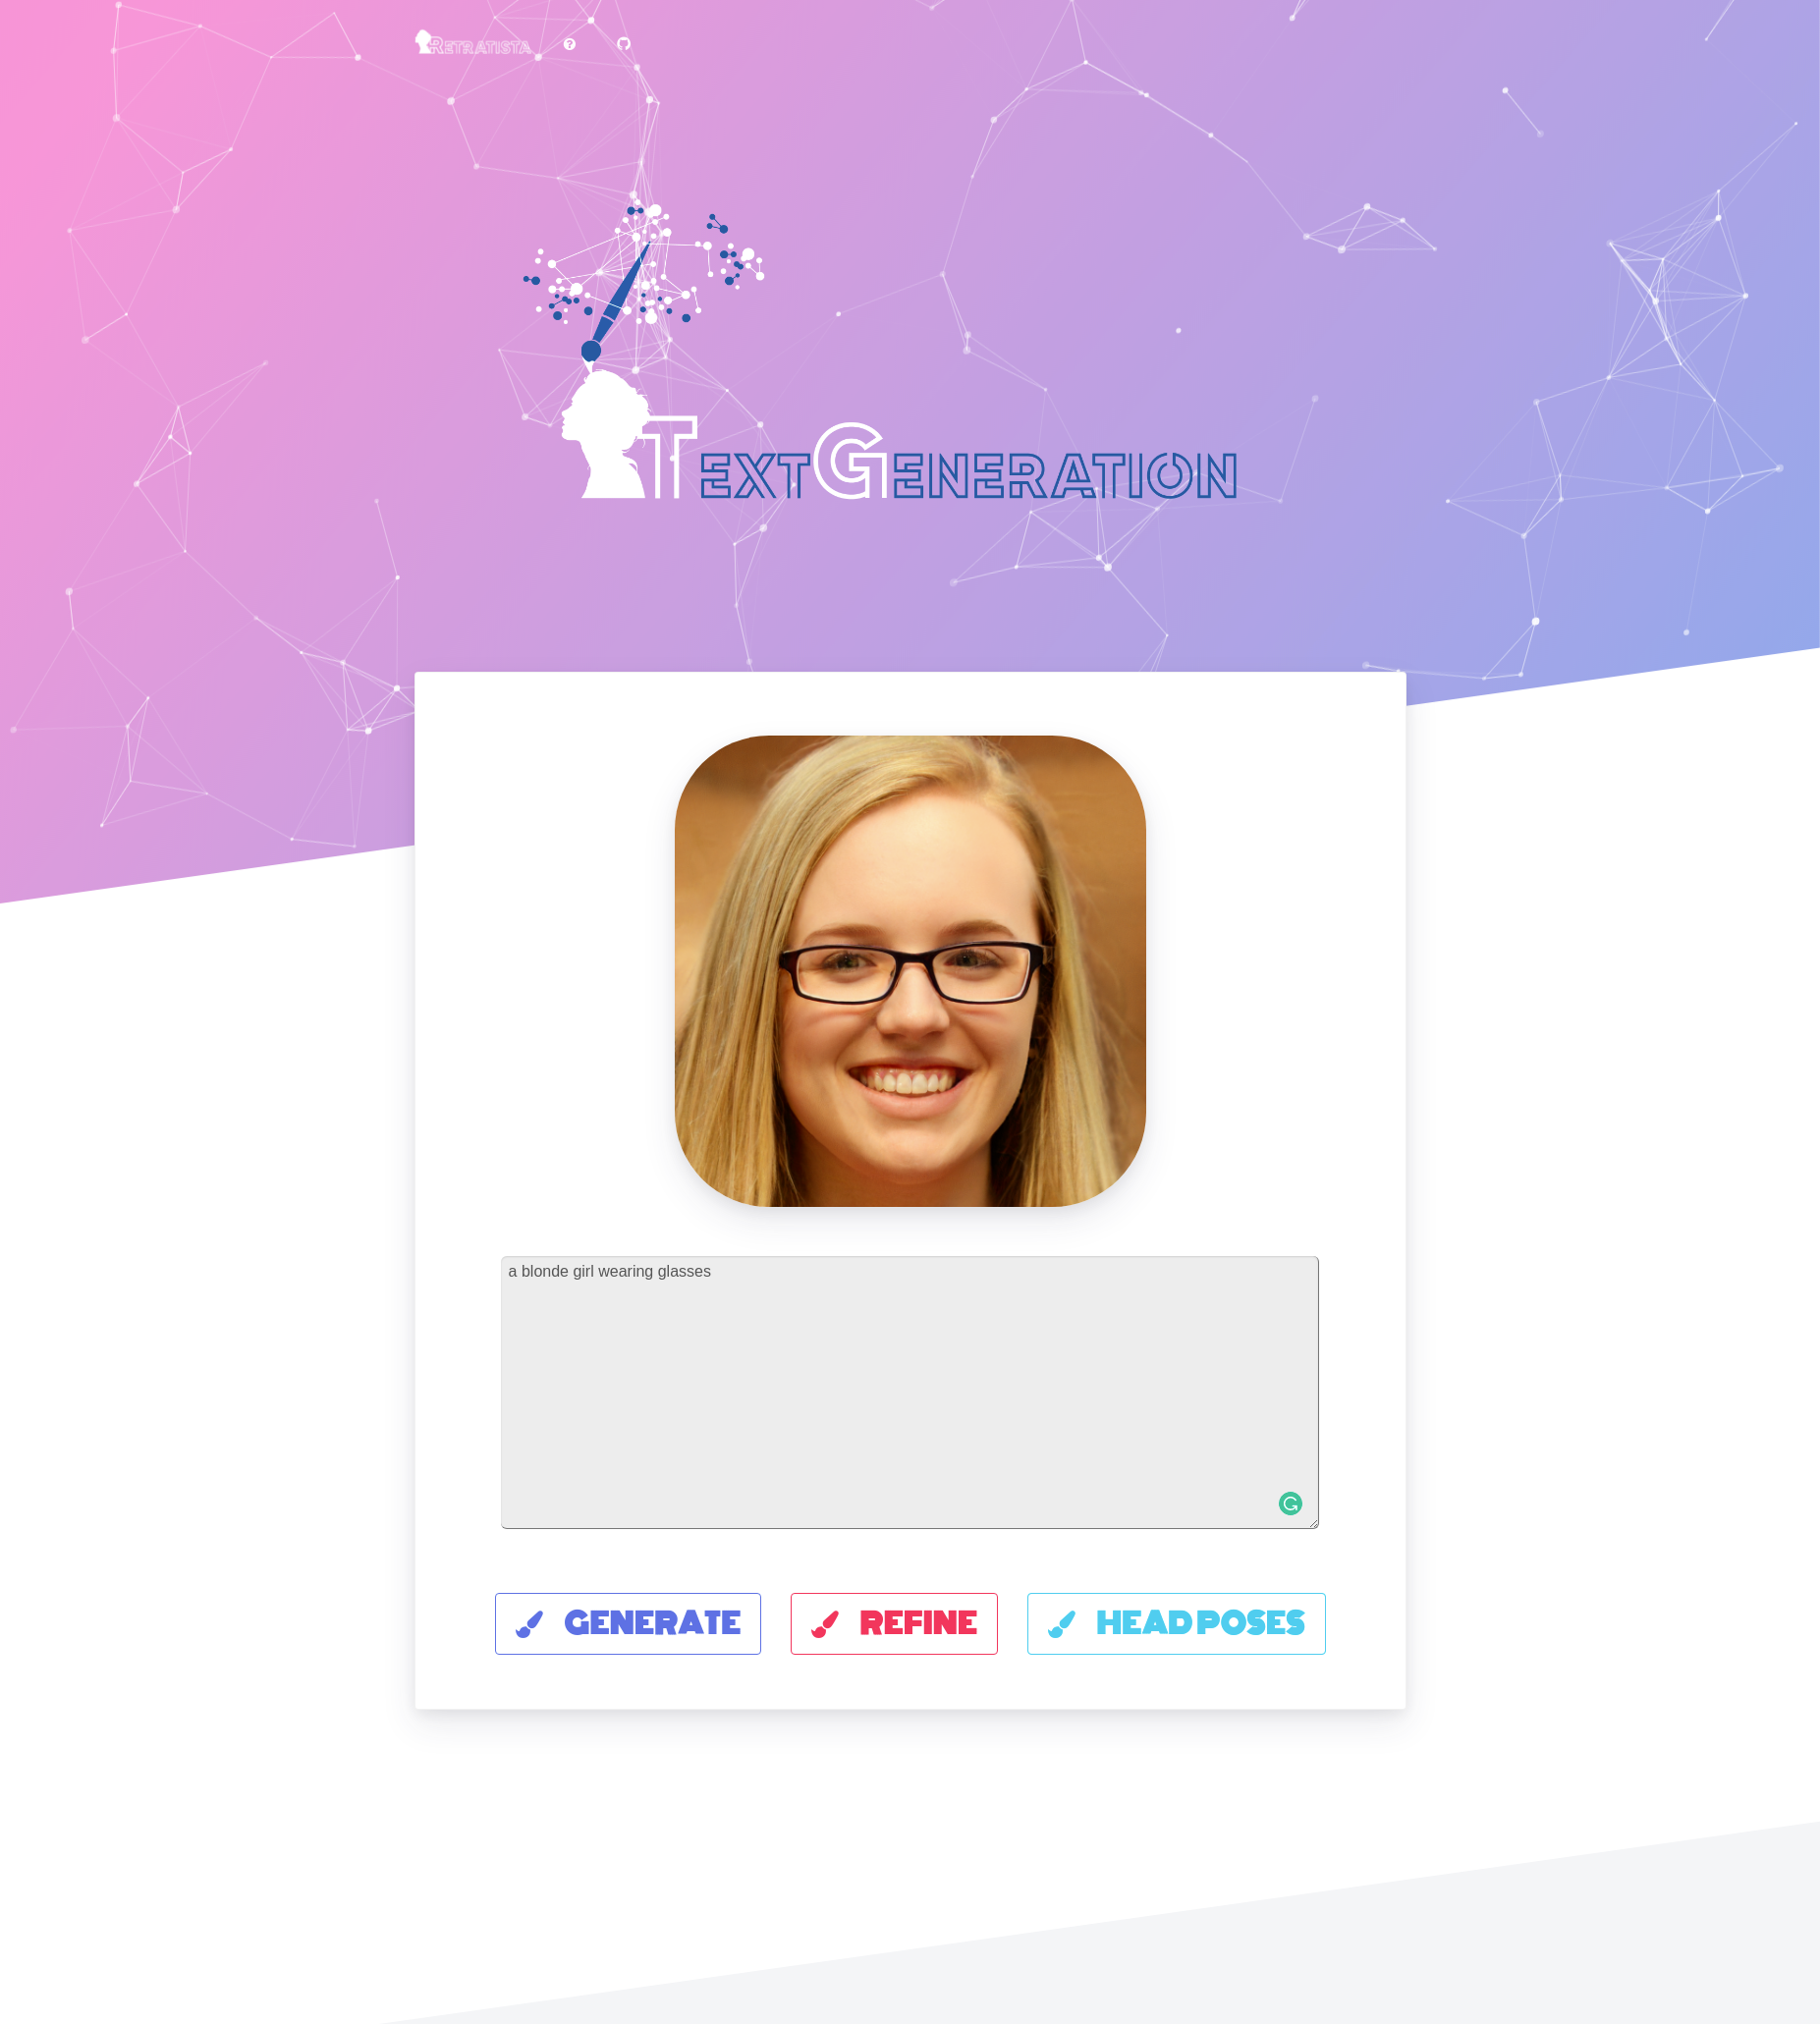
\includegraphics[width=0.7\textwidth]{images/website/text.png}
        \caption{Generation From Textual Description Page}
        \label{fig:text}
    \end{figure}
    
    \item Generation/Refinement Using Manual Manipulators Page
    
    This page allows the user to generate a new face or refine an actually-generated face using maual manipulators, as shown in figure \ref{fig:refine}
    
    \begin{figure}[H]
        \centering
        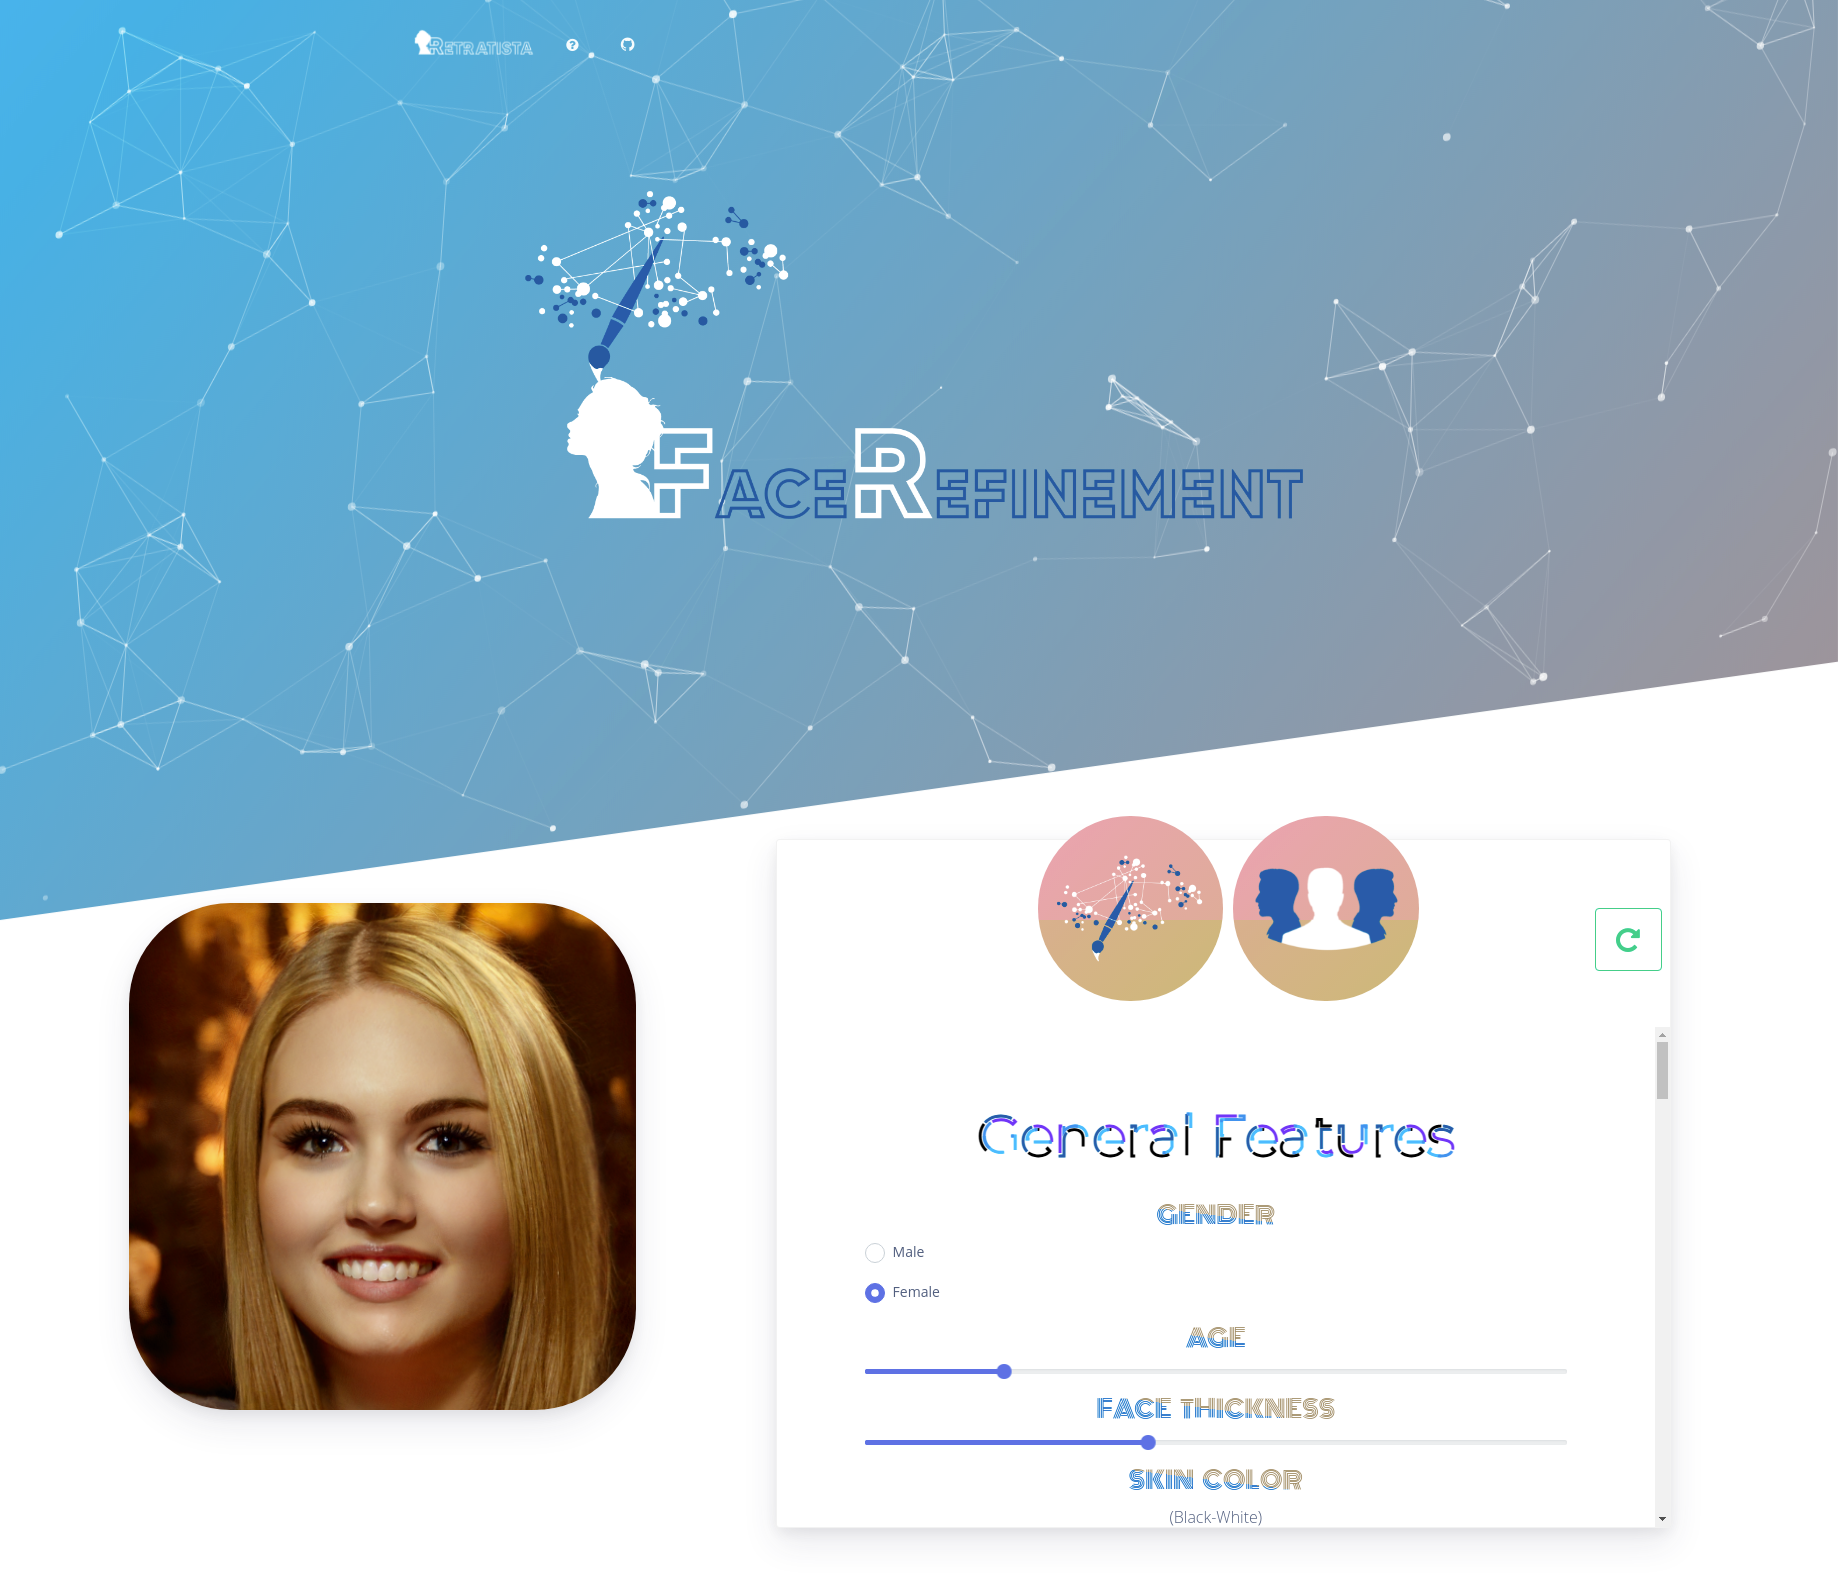
\includegraphics[width=0.7\textwidth]{images/website/refine1.png}
        \caption{Generation/Refinement Using Manual Manipulators Page}
        \label{fig:refine}
    \end{figure}
    
    \item Head Poses Page
    
    This page generates eight different head poses for extra identification, as shown in figure \ref{fig:poses}
    
    \item Help and Demo Page 
    
    This Page is a help aid for the user to know how to use the application and to support the user with some extra information about the project, such as
    \begin{itemize}
        \item Why is Retratista important?
        \item Statistics
        \item Project Features
        \item How To Use?
        \item Result Samples
        \item Team
    \end{itemize}
    
    \begin{figure}[H]
        \centering
        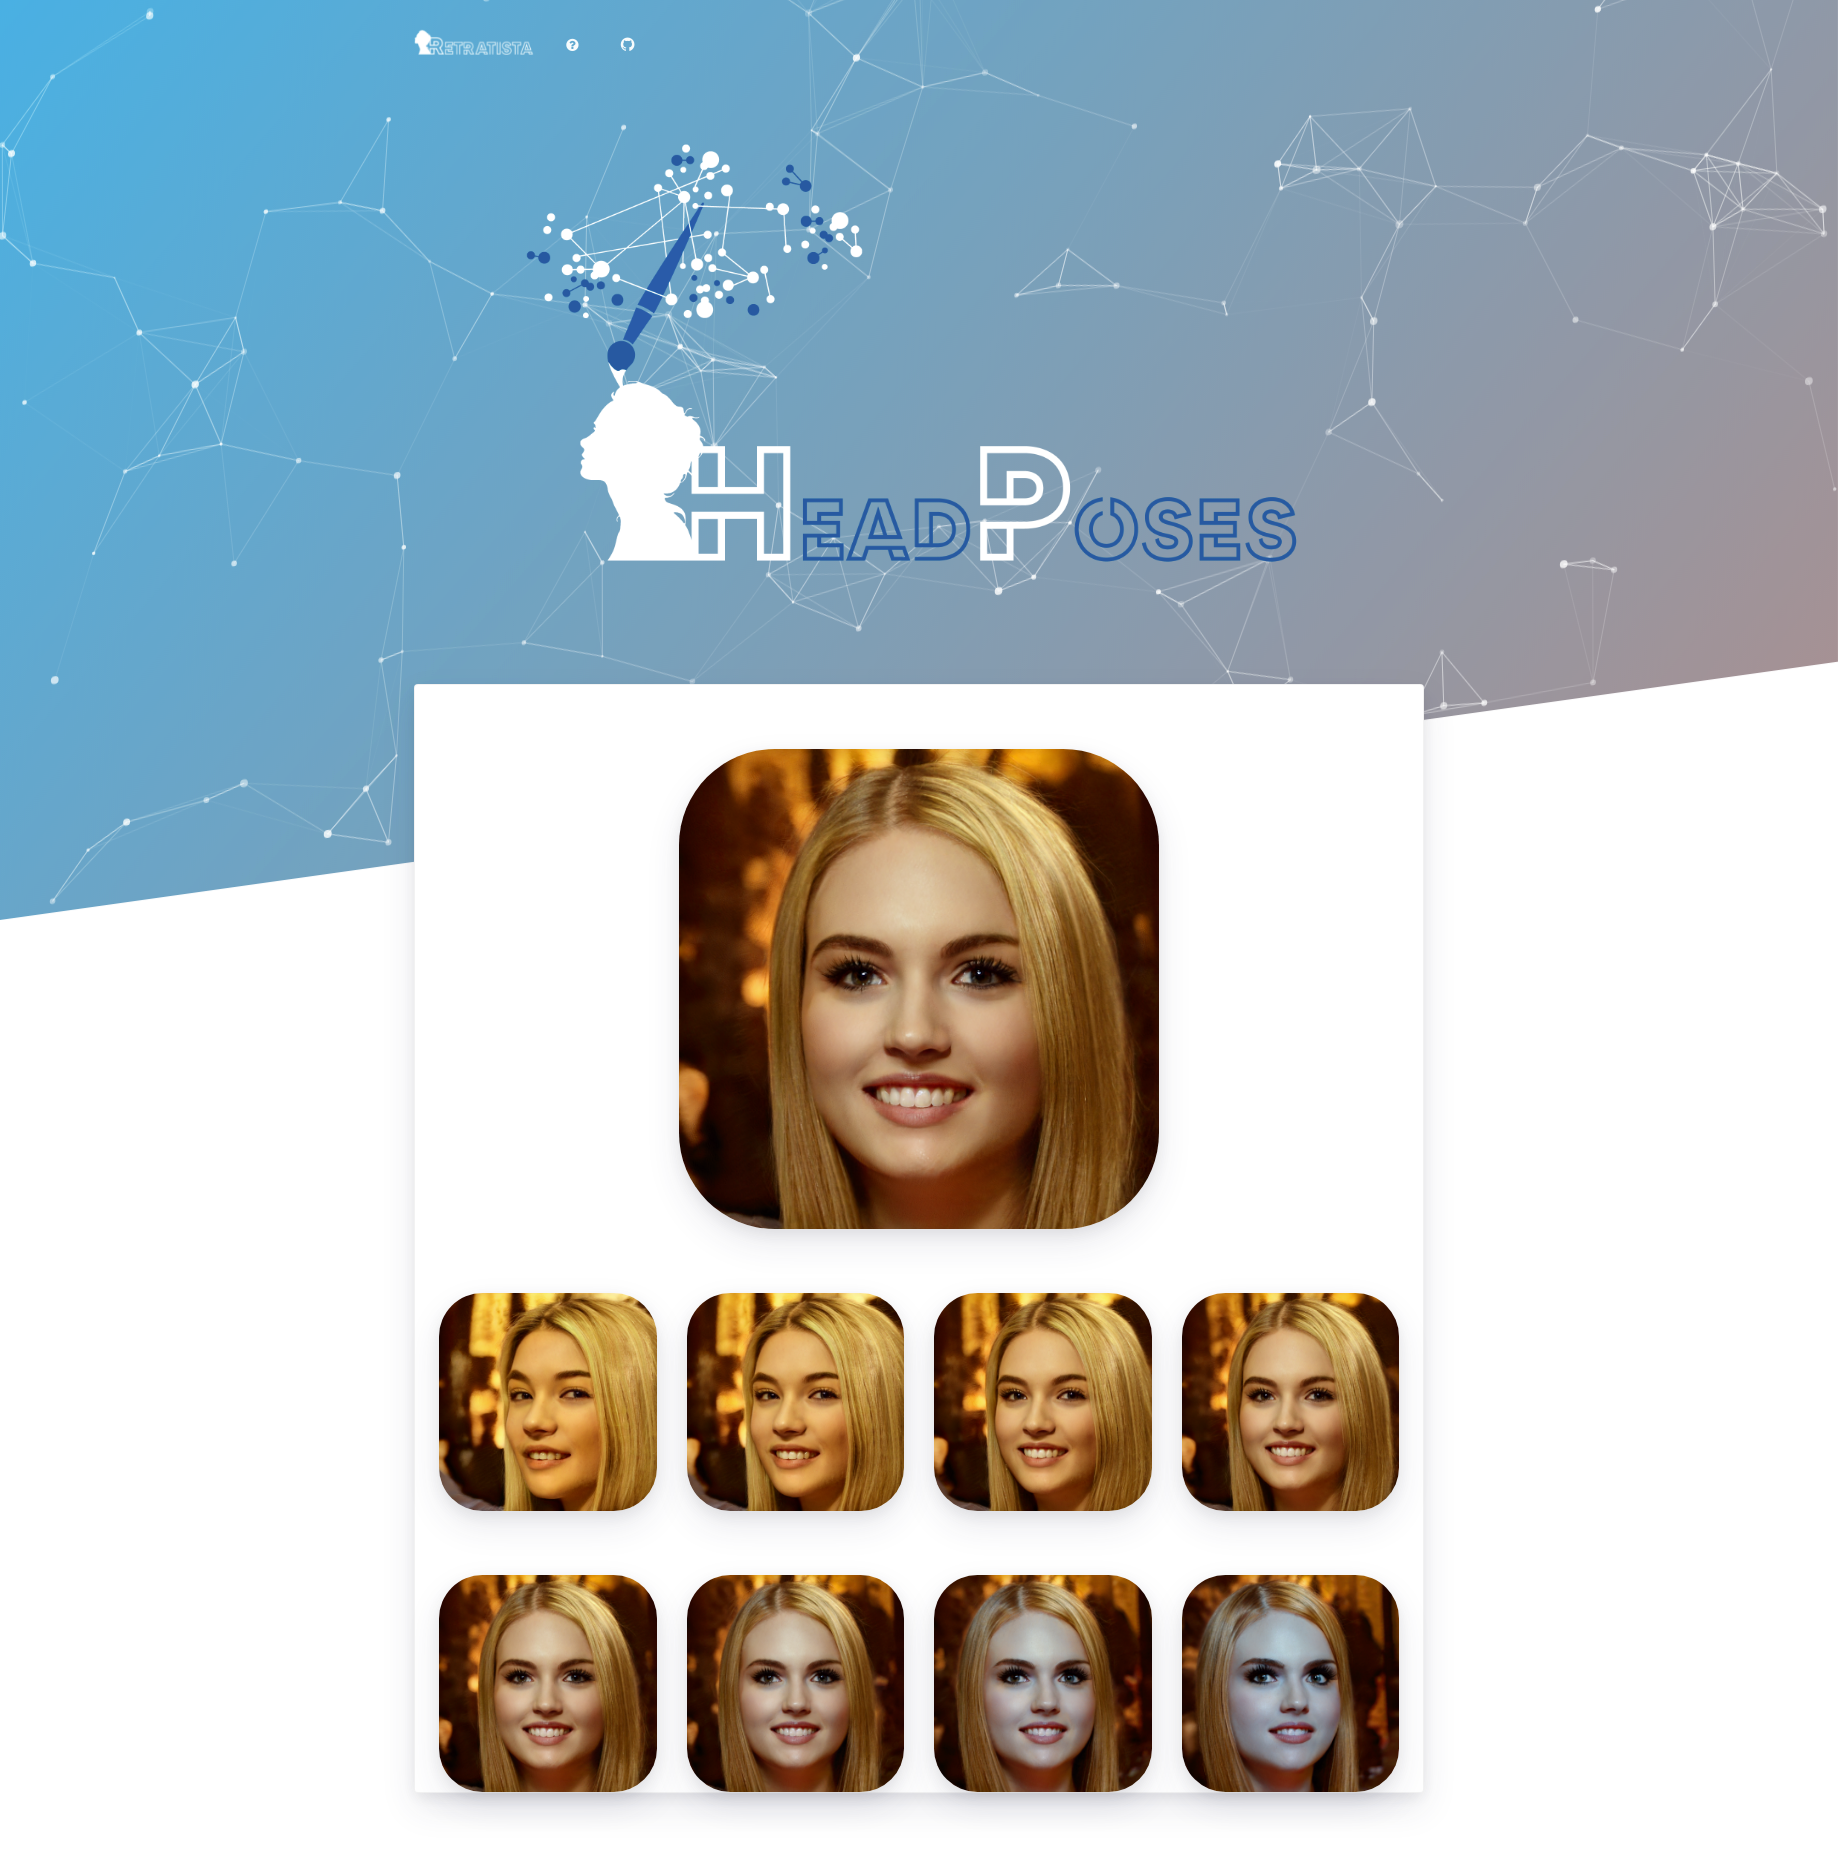
\includegraphics[width=0.7\textwidth]{images/website/poses.png}
        \caption{Head Poses Page}
        \label{fig:poses}
    \end{figure}
    
\end{itemize}

\paragraph{Backend API}
The application backend (shown in \ref{fig:app}) is an \emph{HTTP REST API} that offers $4$ endpoints for all system functionalities. It is composed of $2$ servers communicating through \emph{TCP} ports :
\begin{itemize}
    \item \textbf{StyleGAN Server} : which offers the face generation from description and face refinement functionalities.
    \item \textbf{Pose Server} : which offers the face rotation functionality.
\end{itemize}

The \emph{API} endpoints are listed as follows :
\begin{itemize}
    \item \textbf{Face Generation from Text} :
    \begin{itemize}
        \item \textbf{Request} : textual description (user input or from speech).
        \item \textbf{Response} : face image (portrait) \& numerical attributes values.
    \end{itemize}
    \item \textbf{Face Generation from Values} :
    \begin{itemize}
        \item \textbf{Request} : numerical attributes values (user input).
        \item \textbf{Response} : face image (portrait) \& numerical attributes values.
    \end{itemize}
    \item \textbf{Face Refinement} :
    \begin{itemize}
        \item \textbf{Request} : updates of numerical attributes values (user input).
        \item \textbf{Response} : refined face image (portrait) \& numerical attributes values.
    \end{itemize}
    \item \textbf{Face Poses Generation} :
    \begin{itemize}
        \item \textbf{Request} : angle of rotation (user input).
        \item \textbf{Response} : rotated face image (portrait).
    \end{itemize}
\end{itemize}

\subsubsection{Design Constraints}
As described above, the main constraints on this module are :

\begin{itemize}
    \item Simplicity of User Interface.
    \item Isolation of Complex Techniques used in background.
\end{itemize}
